% Copyright (C) 2009 Thomas L. Kula
% All Rights Reserved
%
% See the file LICENSE for license terms.
\documentclass[12pt]{article}
\usepackage{graphicx}
\setlength{\paperwidth}{5.5in}
\setlength{\paperheight}{8.5in}
\setlength{\textheight}{7.95in}
\setlength{\topmargin}{-0.5in}
\setlength{\oddsidemargin}{-0.5in}
\setlength{\evensidemargin}{-0.5in}
\setlength{\textwidth}{4.0in}
\setlength{\parindent}{0in}
\setlength{\parskip}{3mm}
\usepackage[print]{booklet} \nofiles
\source{\magstep0}{5.5in}{8.5in}
\target{\magstep0}{11in}{8.5in}
\setpdftargetpages
\pagestyle{empty}
\begin{document}



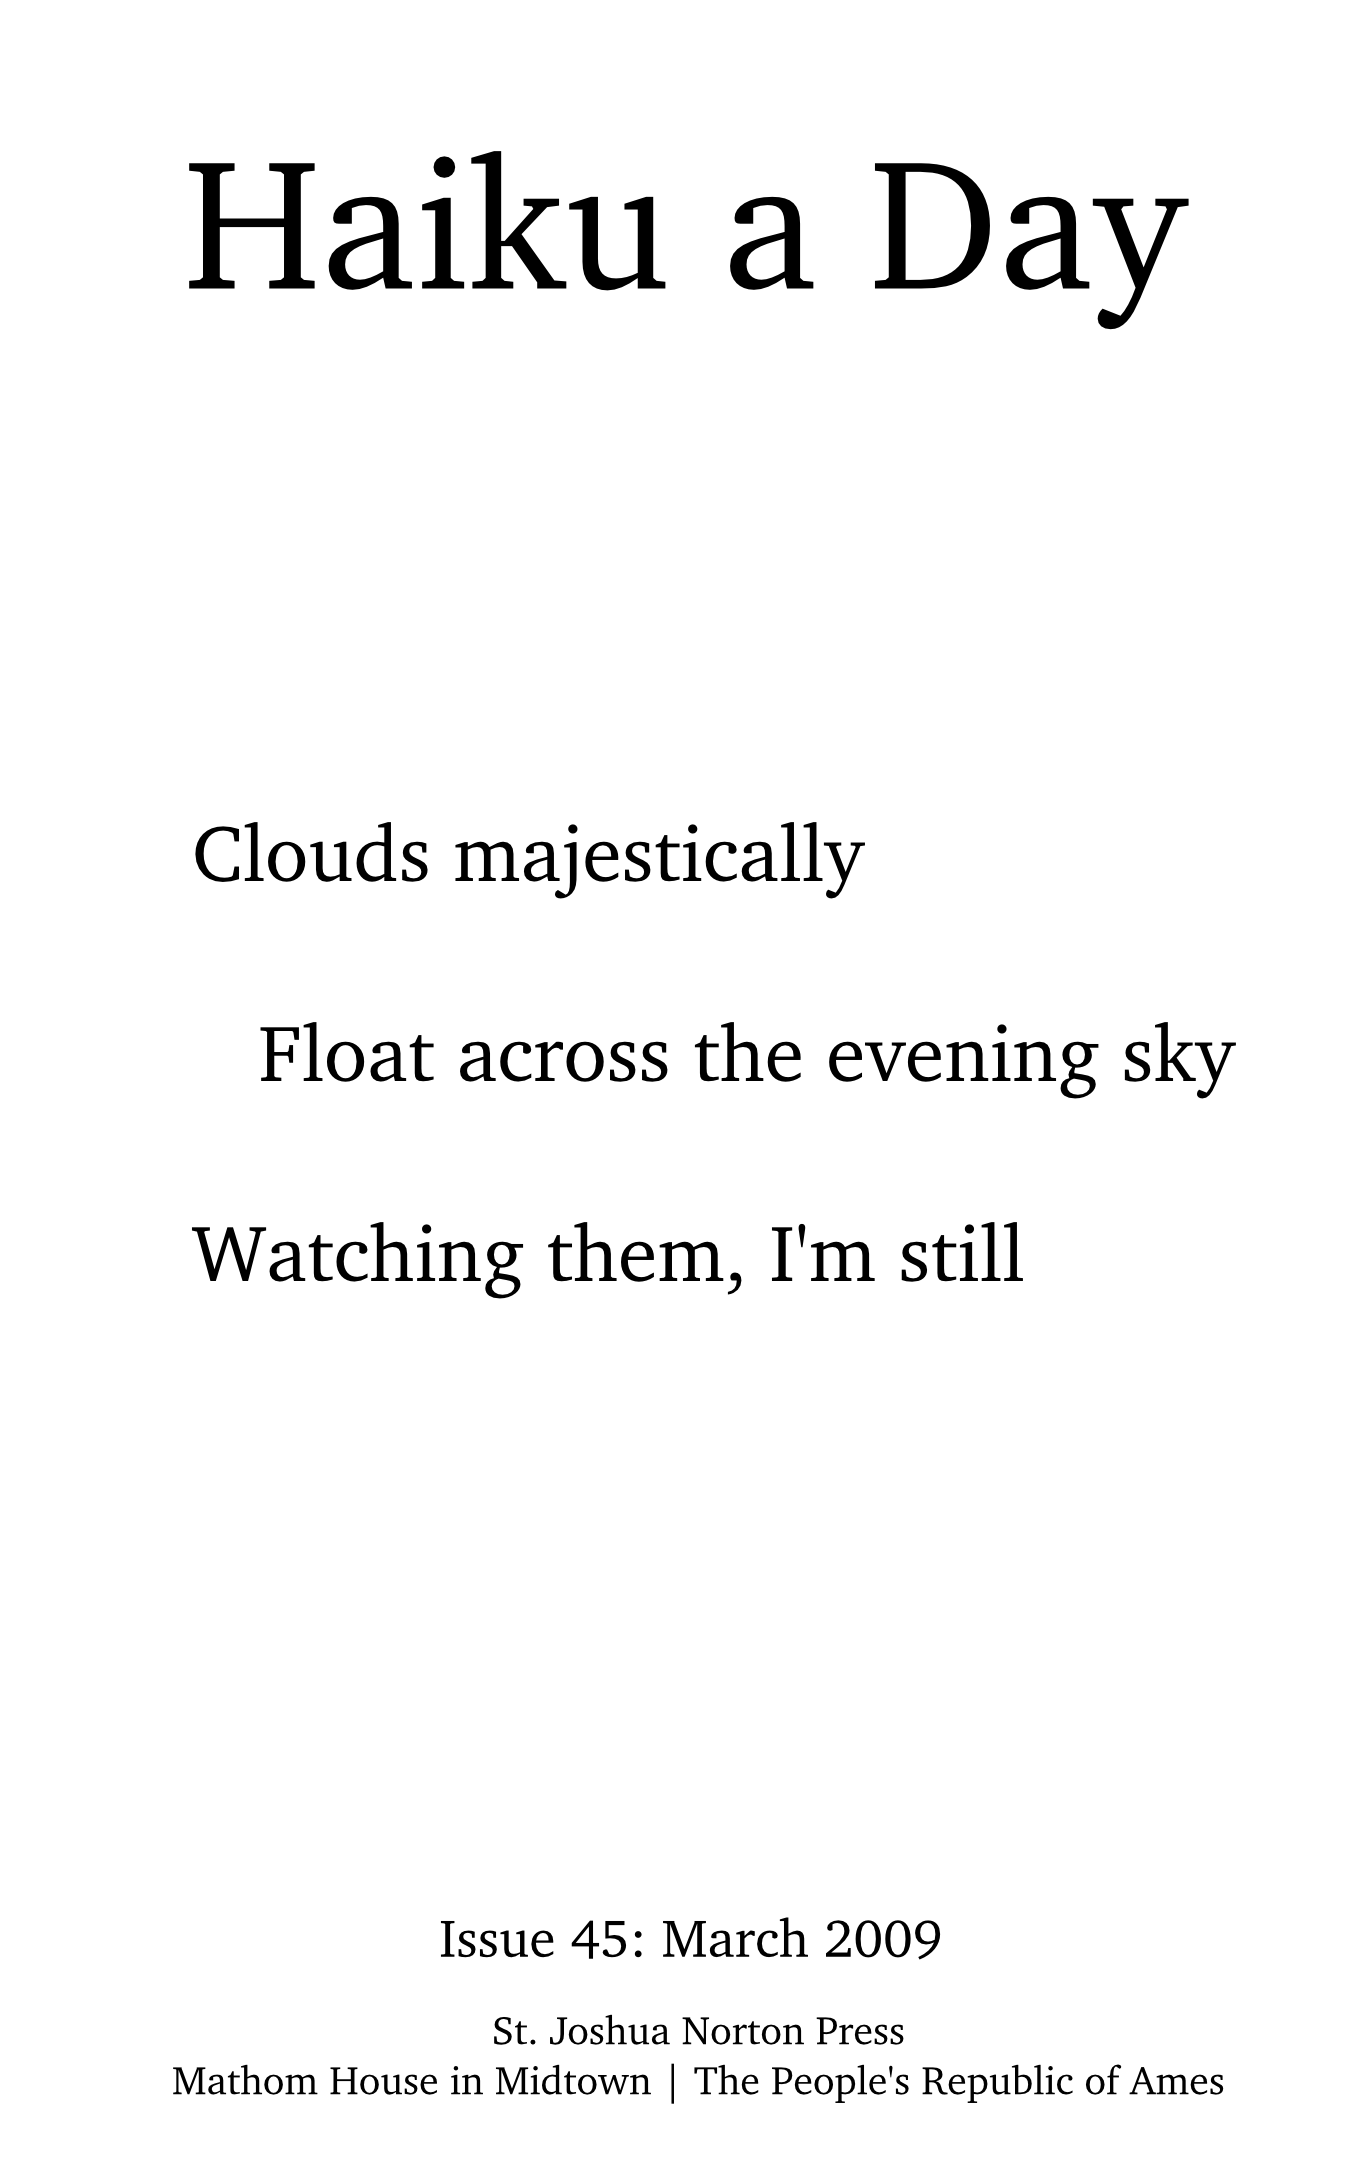
\includegraphics{frontpage.png}

\newpage

I'm off to Chicago tomorrow, but tonight, it's all haiku.
Well, that, and laundry.

--- Thomas

http://kula.tproa.net/had/ \\
kula@tproa.net

Download this and previous HADs at the website, so you can
print out you own (DIY, yeah!) or if you want me to send
you one, send me your address, and maybe a stamp if you
are feeling nice. Or send me something you've made ---
trades always appreciated, postcards are nice too.

1 March 2009

Hidden highways snake \\
Passages long lost to light \\
Where does that vent go?

2 March 2009

Time flies left unwatched \\
Observed slows to a dead crawl \\
Don't look and work ends

\newpage

3 March 2009

Brain wandering on \\
Tuesday nothing to do day \\
It snaps, I go off

4 March 2009

The gaze through the screen \\
Interrupted by old smears \\
I need to clean it

5 March 2009

First class lever sharp \\
Slides through paper in a snap \\
I salute scissors

6 March 2009

Open bottles quick \\
Flick of the wrist, second class \\
Ease of use abounds

7 March 2009

The lever third class \\
A stick, some bristles, and work \\
A sweeping idea

8 March 200

A rock in my shoe \\
How do those ever get in? \\
My mind is baffled

\newpage

9 March 2009

Solid sand gets snapped \\
Two halves and some sharp shards fall \\
I need a new plate

10 March 2009

A walk in the rain \\
Water flowing past my feet \\
The streets glistening

11 March 2009

The skies above clear \\
The wind, emboldened, screaming \\
Shouting out my name

12 March 2009

In a funk walking \\
A coney beckons, plate lands \\
Happy for a bit

13 March 2009

The rains are gone but \\
The ground is still squishy wet \\
Shoes keep my toes dry

14 March 2009

Hold a rope at one \\
Go around the circle full \\
Twice pi you have gone

\newpage

15 March 2009

Ten folks bike polo \\
The sun shining the day warm \\
Outside is so good

16 March 2009

On nights like tonight \\
I feel like my apartment \\
Is just for my stuff

17 March 2009

On a cool spring night \\
Idiots drunk and braying; \\
I bike around them

18 March 2009

A spiral quickens \\
Steel held back fully released \\
The recliner sighs

19 March 2009

I almost stay home \\
Too many meetings today \\
I leave early, though

20 March 2009

Oh sweet! I'm Sick Tea! \\
Tea, lemon, ginger, honey \\
Good for what ails ya!

\newpage

21 March 2009

I sleep the day through \\
And read Wikipedia \\
Sometimes, I find food

22 March 2009

My laptop is full \\
There's no more room for stickers \\
Need another one

23 March 2009

Ears full, my humming \\
Resonates inside my head \\
An organ for me

24 March 2009

The doctor's office \\
Nurse gags me with a q-tip \\
At least it's not strep

25 March 2009

Back to work today \\
Still out of it, but better \\
Flee the apartment

26 March 2009

A knot I don't know \\
The instructions don't make sense \\
My mind is tied up

\newpage

27 March 2009

Alluring popcorn \\
Complex in simplicity \\
Corn heat salt and eat

28 March 2009 

Ears plugged, sounds muffled \\
The grocery store in a daze \\
Need more apple juice

29 March 2009

What soft from the sky \\
Falls upon the late March ground? \\
Snow, for one last turn

30 March 2009

Blue and white tiles \\
A sign of sanitation \\
Cleanliness abounds

31 March 2009

How does it grow right? \\
The skin of an apple fits \\
The fruit perfectly

\newpage


\includegraphics{backpage.png}

\end{document}




